\documentclass[10pt]{article}%{scrartcl} % Beginn der LaTeX-Datei
\usepackage[utf8]{inputenc}  % für Unix-Systeme
\usepackage{amsmath,amssymb,mathtools}  % erleichtert Mathe 
\usepackage{tabularx}
\usepackage{enumerate}% schicke Nummerierung
\usepackage{geometry}
\geometry{a4paper,left=30mm,right=30mm, top=3cm, bottom=2cm} 
\usepackage{graphicx} % für Grafik-Einbindung
%\usepackage[dvips]{hyperref}
\usepackage{mdwlist}
\usepackage[labelfont=bf]{caption}
\usepackage{subcaption}

\usepackage[ngerman]{babel}
\addto\captionsngerman{\renewcommand{\figurename}{Abb.}}
%\usepackage[T1]{fontenc}
%\usepackage{lmodern}
 % Einstellungen, wenn man deutsch schreiben will, z.B. Trennregeln
  % ermöglicht die direkte Eingabe von Umlauten und ß
  % evt. obige Zeile ersetzen durch
  % \usepackage[utf8]{inputenc}
  % \usepackage[ansinew]{inputenc}  % für Windows
  % \usepackage[applemac]{inputenc} % für den Mac

%%%%%%%%%%%%%%%%%%%%%%%%%%%%%%%%%%%%%%%%%%%%%%%%%%%%%%%%%%%%%%%%%%
%
%  ntheorem
%
\usepackage[thmmarks,amsmath,hyperref,noconfig]{ntheorem} 
  % erlaubt es, Sätze, Definitionen etc. einfach durchzunummerieren.
\newtheorem{satz}{Satz}[section] % Nummerierung nach Abschnitten
\newtheorem{hilfssatz}[satz]{Hilfssatz}
\newtheorem{kor}[satz]{Korollar}

\theorembodyfont{\upshape}
\newtheorem{beispiel}[satz]{Beispiel}
\newtheorem{bemerkung}[satz]{Bemerkung}
\newtheorem{definition}[satz]{Definition}

\theoremstyle{nonumberplain}
\theoremheaderfont{\itshape}
\theorembodyfont{\normalfont}
\theoremseparator{.}
\theoremsymbol{\ensuremath{_\blacksquare}}
\newtheorem{beweis}{Beweis}
\qedsymbol{\ensuremath{_\blacksquare}}
%\theoremclass{LaTeX}
%
% Ende ntheorem
%
%%%%%%%%%%%%%%%%%%%%%%%%%%%%%%%%%%%%%%%%%%%%%%%%%%%%%%%%%%%%%%%%%%

%\pagestyle{empty}
%
% Ändern der bedruckten Fläche der Seite
% \addtolength{\textwidth}{3cm}  % Befehl mit zwei Argumenten
% \addtolength{\textheight}{3cm}
% \hoffset-2cm % verschiebt das Textfenster nach links
% \voffset-5mm % verschiebt das Textfenster nach oben
%
%\parindent=0pt %% keine Einzug zu Beginn von Abs\"atzen
%\parskip=2mm   %% erzeugt einen zusätzliche Zeilenabstand zwischen
                %% Absätzen. Nötig bei \parindent=0pt


\usepackage{pgf}
\usepackage{tikz}
\usetikzlibrary{arrows,automata,calc,patterns,positioning,shapes}


%%%%%%%%%%%%%%%%%%%%%%%%%%%%%%%%%%%%%%%%%%%%%%%%%%%%%%%%%%%%%%%%%%
%
%  ermöglicht, farbigen Text zu drucken.
%
\usepackage{color}
% Und nun werden die Farben definiert - daran können Sie nach Belieben selber rumspielen.
\definecolor{white}{rgb}{1,1,1}
\definecolor{darkred}{rgb}{0.3,0,0}
\definecolor{darkgreen}{rgb}{0,0.3,0}
\definecolor{darkblue}{rgb}{0,0,0.3}
\definecolor{pink}{rgb}{0.78,0.09,0.51}
\definecolor{purple}{rgb}{0.28,0.24,0.55}
\definecolor{orange}{rgb}{1,0.6,0.0}
\definecolor{grey}{rgb}{0.4,0.4,0.4}
\definecolor{aquamarine}{rgb}{0.4,0.8,0.65}


\DeclareMathOperator{\GL}{GL} % einige Macro, siehe am Ende Abschn. 2
\newcommand{\N}{\mathbb{N}}
\newcommand{\Z}{\mathbb{Z}}
\newcommand{\Q}{\mathbb{Q}}
\newcommand{\R}{\mathbb{R}}
\newcommand{\PP}{\mathbb{P}}
\newcommand{\PPX}{\mathbb{P}^X}
\newcommand{\C}{\mathbb{C}}
\newcommand{\cP}{{\mathcal P}} 

\setlength{\parindent}{0cm}
\setlength{\parskip}{.2cm}
\setlength{\fboxsep}{0pt}
%\setlength{\fboxrule}{.2mm}

%\usepackage{showframe}

\begin{document}

\author{Gruppe 04 -- Alex Oks, Markus Görlich, Simon Stieber}
\title{Selbstorganisierende, adaptive Systeme - Blatt 04}
%\date{} %hier können Sie ein Datum eingeben, auch leer, sonst wird es
         %automatisch erzeugt

\maketitle % erzeugt den Kopf
%%\let\clearpage\relax

\section{Aufgabe 3 - Entwurf Simon}
Formale Definition von Spielen: (Skript Nr. 4 F. 16):\\
Ein strategisches Spiel $G = \langle N, (A_i )_{i \in N} , (u_i )_{i \in N}\rangle$ besteht aus
\begin{itemize}
	\item einer endlichen Menge N = 1,..., n an Spielern
	\item einer Menge an Aktionen $A_i$ für jeden Spieler
	\item einer Nutzenfunktion (utility) $u_i$ : $A_1  \times ... \times A_n \rightarrow R$ für jeden
	Spieler
\end{itemize}
\subsection{a}
Wenden Sie die formale Definition an, um die Entscheidungssimulation zu modellieren.
Hier:
\begin{itemize}
	\item $N$: Computer in einem Netzwerk
	\item $A_i$: Datei im Cache behalten oder Datei anfordern
	\item $u_i$: Die Nutzenfunktion ergibt sich aus den Kosten für Anfordern oder Behalten 
\end{itemize}

\subsection{b}
Bestimmen Sie die weiteren Nash-Gleichgewichte (nur in reinen Strategien) in Abbildung 1.
\begin{itemize}
	\item Nash Gleichgewicht:
	Für jeden Agenten i = 1, . . . , n gilt, dass $u_i(a) \geq u_i ((a_{-i} , a )) \forall a \in A_i$
	\item Reine Strategie: Immer nur eine Aktion wählen
\end{itemize}
\emph{TODO} Kann ich mir noch keinen richtigen Reim drauf machen, was da alles mit was verglichen werden muss.
Habs versucht zu skizzieren, aber bin noch nicht ganz durchgestiegen.

\subsection{c}
\emph{TODO}
Skizze: siehe Abb. \ref{skz3c}
\begin{figure}
	\centering
	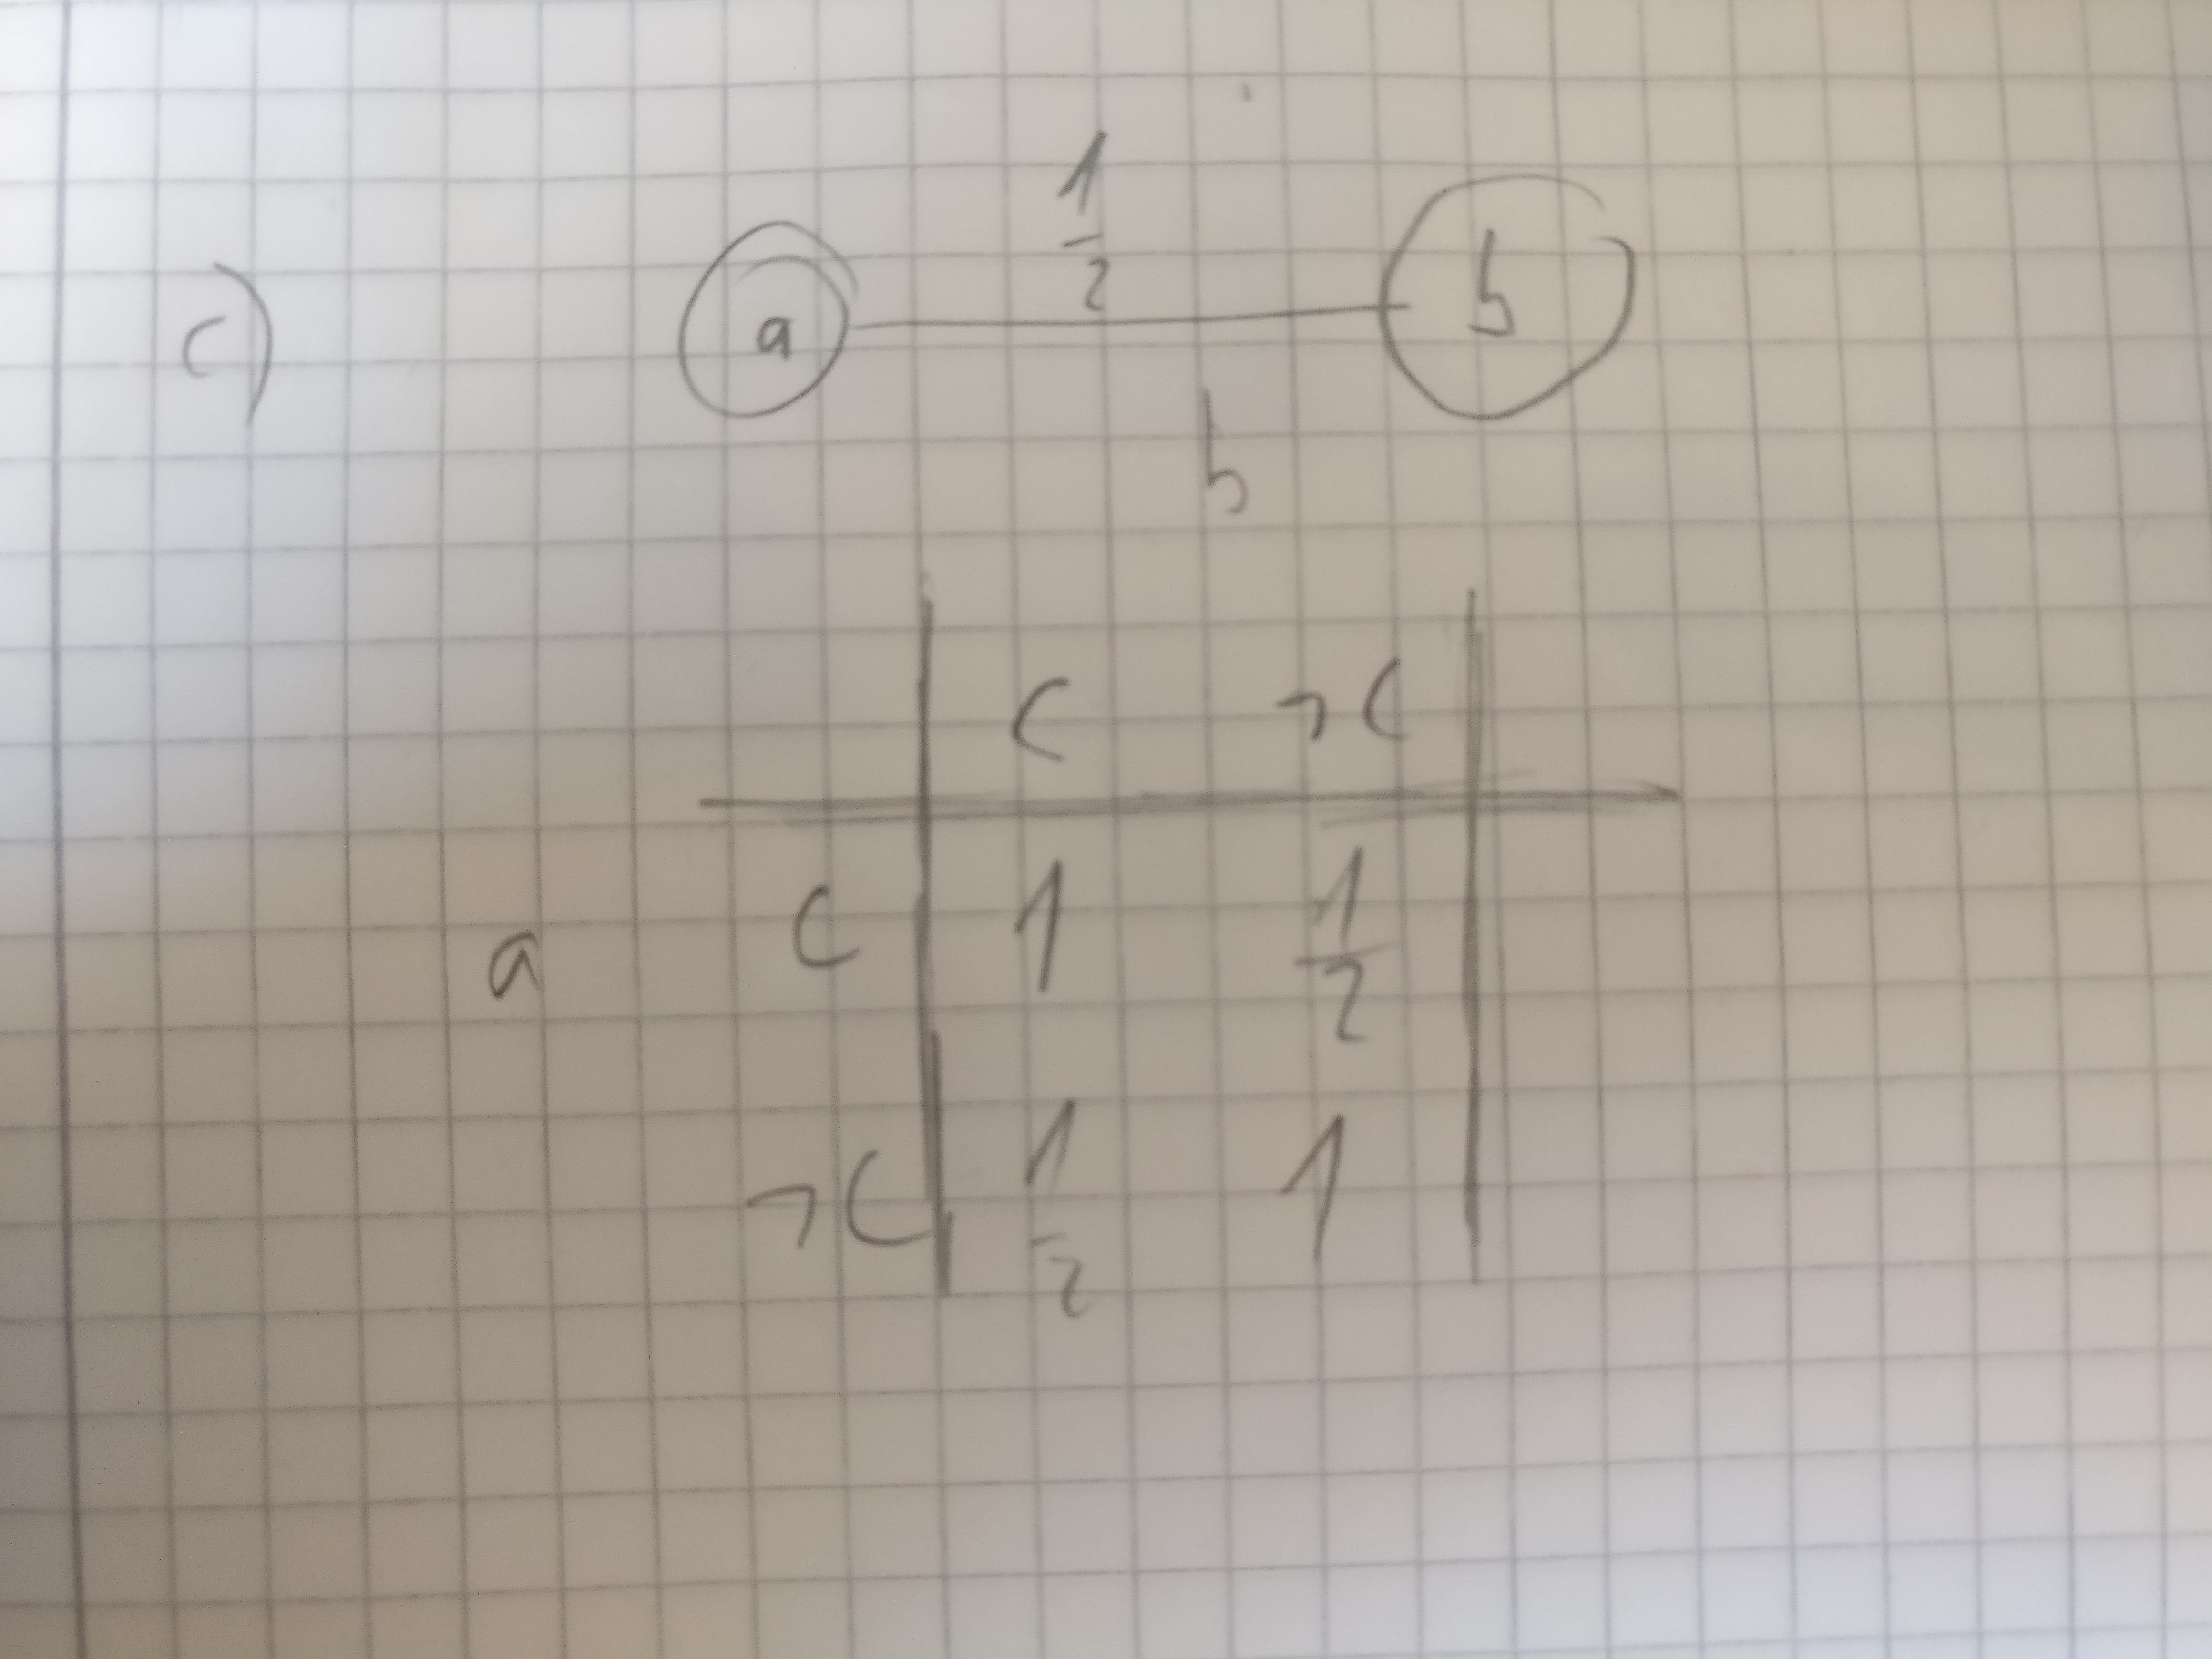
\includegraphics[width=0.5\textwidth]{img/Skizze3c.jpg}
	\caption{Skizze zu 3c}
	\label{skz3c}
\end{figure}

\subsection{d}
Untersuchung Algorithmus:\\
Durchgänge:
\begin{enumerate}
	\item i = b, weil d(i) = 3. $S=\{b\}$, $N=\{a,c,d,e,f\} \rightarrow N=\{c, e\}$
	\item i = c oder e, weil d(c)=2, d(e)=2. Wähle c. $S=\{b, c\}$, $N=\{e\} \rightarrow N=\{e\}$
	\item Dasselbe passiert bei der Wahl von e $\rightarrow$ Gleichgewicht $S=\{b, c, e\}$
\end{enumerate}
Erzeugt dieser Algorithmus stets ein Nash Gleichgewicht?
Zum Schluss bleiben immer Knoten $S$ übrig, die cachen sollen.
Ist das immer ein Gleichgewicht?
TODO
\end{document}